\documentclass[a4paper]{article}
\usepackage[utf8]{inputenc}
\usepackage[left=2.5cm,right=2.5cm,top=2.5cm,bottom=2.5cm]{geometry}
\usepackage{amsmath}
\usepackage{amsfonts}
\usepackage{amssymb}
\usepackage{graphicx}
\usepackage{fancyhdr}
\usepackage{titlesec}
\usepackage{enumitem}
\usepackage{booktabs}
\usepackage{longtable}
\usepackage{url}
\usepackage{abstract}
\usepackage{caption}
\usepackage{scrextend} % For arbitrary font sizes
\changefontsizes{13pt} % Set exactly 13pt font size

% Header configuration
\pagestyle{fancy}
\fancyhf{}
\renewcommand{\headrulewidth}{0.5pt}
\lhead{\small Molecular Biology And Genetics Laboratory, Department of Biotechnology}
\rhead{\small \thepage}
\chead{}
\lfoot{}
\rfoot{}
\cfoot{}

% Section formatting
\titleformat{\section}{\normalfont\Large\bfseries}{\thesection.}{0.5em}{}
\titleformat{\subsection}{\normalfont\large\bfseries}{\thesubsection.}{0.5em}{}
\titleformat{\subsubsection}{\normalfont\normalsize\bfseries}{\thesubsubsection.}{0.5em}{}

% Customizing the title section
\makeatletter
\renewcommand{\@maketitle}{
    \noindent
    \begin{minipage}[c]{0.1\textwidth}
        
\includegraphics[width=40px]{Images/bachkhoa_logo.png}
    \end{minipage}%
    \begin{minipage}[c]{0.9\textwidth}
        \quad Ho Chi Minh City University of Technology (HCMUT), VNU-HCM
    \end{minipage}
    \par
    \vskip 0.5em
    \hrule
    \vskip 2em
    \begin{center}
    {\huge\bfseries MOLECULAR BIOLOGY AND GENETICS: \par}
    {\huge\bfseries LABORATORY REPORT \par}
    \vskip 2em
    
    \textit{{\large 
        Dinh Chan Phong\_2352902\textsuperscript{1,2}, 
        Dong Minh Nghia\_2252525\textsuperscript{1,2}, 
        Dinh Nguyen Chinh Nghia\_2352804\textsuperscript{1,2}, 
        Nguyen Tran Nam Nguyen\_2352834\textsuperscript{1,2}, 
        Hoang My Dung\textsuperscript{1,2,*} 
    }} \par
    \vskip 1.5em
    {\small \textsuperscript{1} Department of Biotechnology, Faculty of Chemical Engineering, Ho Chi Minh City University of Technology (HCMUT) \par}
    {\small \textsuperscript{2} Office for International Study Programs, Ho Chi Minh City University of Technology (HCMUT), 268 Ly Thuong Kiet Street, Dien Hong Ward, Ho Chi Minh City, Vietnam \par}
    \vskip 1em
    {\small * Corresponding author: hoangmydung@hcmut.edu.vn \par}
    \end{center}
}
\makeatother

\begin{document}
\sloppy % Allow more flexible word spacing to avoid hyphenation

\maketitle

\begin{abstract}
This study investigates the biological impact of Ultraviolet (UV) radiation on bacterial genomic integrity through a comprehensive molecular biology workflow. The experimental procedure began with the cultivation of bacteria in liquid MRS medium, followed by controlled UV exposure for 30 minutes to induce DNA damage. To assess cellular recovery and genetic stability, DNA was extracted using the Trizol-chloroform method across varying post-exposure incubation intervals. The extracted genetic material was subsequently analyzed via Polymerase Chain Reaction (PCR) and Agarose Gel Electrophoresis to evaluate the success of DNA recovery and the extent of UV-induced modifications. This integrated approach provides a practical framework for understanding DNA damage mechanisms and the fundamental techniques of genetic analysis, bridging the gap between theoretical molecular biology and laboratory application.
\end{abstract}

\noindent\textbf{Keywords:} UV radiation; DNA extraction; Trizol method; PCR; Electrophoresis; Bacterial DNA integrity.

\vskip 2em
\hrule
\vskip 2em

\section{Introduction}
In the field of molecular biology, the ability to isolate, amplify, and analyze genetic material is a foundational requirement for both research and diagnostic applications. Among the various environmental factors affecting genetic stability, Ultraviolet (UV) radiation serves as a primary mutagenic agent capable of inducing structural lesions in DNA. Understanding how these stressors impact microbial genomes is essential for studying DNA repair mechanisms and evolutionary biology.

This laboratory series was designed to equip students with essential techniques in molecular genetics while observing the real-time effects of UV-induced stress on bacterial cultures. The workflow encompasses a complete cycle of molecular analysis:
\begin{itemize}
    \item Bacterial Cultivation: Establishing a robust biomass in MRS medium at 37$^\circ$C.
    \item Mutagenic Treatment: Subjecting the samples to UV exposure and monitoring recovery phases.
    \item Genomic Extraction: Utilizing the Trizol reagent protocol to isolate high-quality DNA through organic phase separation and centrifugation at 12000g.
    \item Molecular Characterization: Employing PCR amplification and agarose gel electrophoresis at 110mV to visualize and verify the targeted DNA segments.
\end{itemize}
By integrating these core methodologies, the experiment provides a comprehensive assessment of the impact of physical stressors on bacterial DNA, reinforcing the theoretical principles of molecular genetics through empirical evidence.

\section{Theoretical Background}

\subsection{UV-Induced DNA Damage and Repair}
Ultraviolet (UV) radiation, particularly in the UV-C (200--280 nm) and UV-B (280--320 nm) ranges, is a potent mutagen that causes direct damage to DNA. The most common lesions are cyclobutane pyrimidine dimers (CPDs) and 6-4 photoproducts, formed between adjacent pyrimidine bases (cytosine or thymine) \cite{1}. These structural distortions interfere with DNA replication and transcription, potentially leading to mutations or cell death. Bacteria have evolved several repair mechanisms, including photoreactivation and nucleotide excision repair (NER), to maintain genomic integrity following UV exposure \cite{1}.

\subsection{Principles of Nucleic Acid Extraction}
The isolation of high-purity genomic DNA is a prerequisite for downstream molecular applications. The Trizol method (acid guanidinium thiocyanate-phenol-chloroform extraction) is a widely used technique for the simultaneous isolation of RNA, DNA, and proteins \cite{2}. Guanidinium thiocyanate acts as a powerful denaturant that lyses cells and inactivates nucleases. The addition of chloroform leads to phase separation: DNA partitions into the interphase or organic phase under acidic conditions, but can be recovered from the organic phase using specialized back-extraction buffers (BEB) which shift the pH to allow DNA solubilization into the aqueous phase \cite{2}.

\subsection{Polymerase Chain Reaction (PCR)}
PCR is an \textit{in vitro} technique for the exponential amplification of specific DNA sequences. The process relies on thermal cycling, consisting of three discrete temperature steps: denaturation (to separate DNA strands), annealing (to allow primers to bind to target sequences), and extension (where a thermostable DNA polymerase, such as Taq, synthesizes new DNA strands) \cite{3}. PCR allows for the detection of even minute quantities of genetic material, making it essential for verifying the presence and integrity of extracted DNA.

\subsection{Agarose Gel Electrophoresis}
Agarose gel electrophoresis is the standard method for separating DNA fragments based on their size and charge. Under an electric field, negatively charged DNA molecules migrate through the porous agarose matrix toward the positive anode \cite{4}. Smaller fragments migrate faster than larger ones, allowing for the determination of fragment sizes when compared against a molecular weight marker (ladder). Visualization is typically achieved using fluorescent dyes, such as GelRed, which intercalate with DNA and fluoresce under UV light \cite{4}.

\section{Materials \& Methods}

\subsection{Bacterial Cultivation and Preparation}
The experimental workflow utilized \textit{Lactobacillus} species as the biological model. Cultures were initiated from a solid-phase inoculum into liquid MRS (de Man, Rogosa, and Sharpe) medium. MRS medium provides a specialized nutrient profile (including acetate and polysorbate 80) that selectively supports the growth of Lactic Acid Bacteria (LAB) while suppressing competitive microflora. Inoculated samples were incubated at 37$^\circ$C for 12 hours to ensure the population reached the late logarithmic growth phase, providing optimal biomass density for downstream genomic isolation.

\subsection{UV Irradiation and Post-Exposure Recovery}
Bacterial suspensions were transferred to sterile, open-lid Petri dishes to avoid UV-C attenuation by plastic. Samples were subjected to direct UV radiation for 30 minutes to induce significant cyclobutane-pyrimidine dimer (CPD) lesions. To evaluate the kinetics of the bacterial DNA repair systems, particularly the nucleotide excision repair (NER) pathway, samples were moved to a dark environment at room temperature (25$^\circ$C) for varying recovery intervals, as detailed in Table 1.

\begin{table}[h!]
\centering
\caption{Post-Exposure Incubation Intervals and Experimental Groups}
\label{tab:uv_intervals}
\begin{tabular}{@{}llcc@{}}
\toprule
\textbf{Group ID} & \textbf{Condition} & \textbf{UV Exposure (min)} & \textbf{Recovery Time (min)} \\ \midrule
Control 1         & Negative Control   & 0                          & 0                            \\
Control 2         & Negative Control   & 0                          & 120                          \\
T1                & UV Treated         & 30                         & 15                           \\
T2                & UV Treated         & 30                         & 30                           \\
T3                & UV Treated         & 30                         & 60                           \\
T4                & UV Treated         & 30                         & 90                           \\
T5                & UV Treated         & 30                         & 120                          \\ \bottomrule
\end{tabular}
\end{table}

\subsection{Genomic DNA Isolation (TRIzol-BEB Method)}
Total genomic DNA (gDNA) was isolated using a modified TRIzol protocol. Unlike standard RNA-focused extractions, this method employs a Back Extraction Buffer (BEB) to recover DNA from the organic/interphase layers.
\begin{enumerate}
    \item \textbf{Biomass Harvesting:} Cells were pelleted via centrifugation at 6000g for 15 minutes.
    \item \textbf{Lysis and Deproteinization:} 1 mL of TRIzol (phenol/guanidine thiocyanate) was added to the pellet. Following a 5-minute incubation, 200 $\mu$L of chloroform was added to facilitate phase separation via vigorous agitation.
    \item \textbf{Phase Partitioning:} Samples were centrifuged at 12000g for 15 minutes at 4$^\circ$C. The upper aqueous phase was discarded. 
    \item \textbf{DNA Back-Extraction:} 500 $\mu$L of alkaline BEB was added to the organic phase. This shifts the pH, allowing the gDNA to transition from the interphase into the new aqueous layer during a 10-minute inversion period.
    \item \textbf{Precipitation:} DNA was precipitated from the recovered aqueous phase using 400 $\mu$L of cold isopropanol, centrifuged at 12000g, and washed with 70\% ethanol to remove residual chaotropic salts. The final pellet was resuspended in 50 $\mu$L of TE buffer.
\end{enumerate}

\subsection{Molecular Characterization via PCR and Electrophoresis}
Targeted DNA sequences were amplified to assess genomic integrity. The PCR reaction was prepared according to the parameters in Table 2, following the thermal cycling profile outlined in Table 3.

\begin{table}[h!]
\centering
\begin{minipage}{0.45\textwidth}
\centering
\caption{PCR Reaction Components}
\label{tab:pcr_mix}
\begin{tabular}{@{}lc@{}}
\toprule
\textbf{Component} & \textbf{Volume ($\mu$L)} \\ \midrule
2X Master Mix      & 10.0                     \\
Forward Primer (5 $\mu$M) & 1.6                      \\
Reverse Primer (5 $\mu$M) & 1.6                      \\
Template DNA       & 1.0                      \\
Nuclease-Free Water & 5.8                      \\ \midrule
\textbf{Total Volume} & \textbf{20.0}            \\ \bottomrule
\end{tabular}
\end{minipage}
\hfill
\begin{minipage}{0.45\textwidth}
\centering
\caption{Thermal Cycling Profile}
\label{tab:pcr_cycle}
\begin{tabular}{@{}lccc@{}}
\toprule
\textbf{Step} & \textbf{Temp ($^\circ$C)} & \textbf{Time} & \textbf{Cycles} \\ \midrule
Initial Denat. & 95 & 15 min & 1 \\
Denaturation   & 95 & 30 s   & \\
Annealing      & 55 & 30 s   & 35 \\
Extension      & 72 & 45 s   & \\
Final Ext.     & 72 & 5 min  & 1 \\ \bottomrule
\end{tabular}
\end{minipage}
\end{table}

The resulting amplicons were analyzed via 1\% agarose gel electrophoresis (0.5 g agarose in 50 mL 1X TAE buffer). Samples (10 $\mu$L) were mixed with 2 $\mu$L of GelRed nucleic acid stain. Electrophoresis was performed at a constant 110 mV for 45 minutes to achieve high-resolution separation of fragments. Bands were visualized using a UV transilluminator and sized against a 100 bp molecular weight ladder.

\section{Results}
The PCR products were analyzed by gel electrophoresis (1\% agarose, 1$\times$ TAE, 110 V, $\sim$35 min, GelRed stain) and visualized under UV transillumination. The resulting banding patterns across the different experimental lanes are summarized in Figure 1 and Table 4.

\begin{figure}[h!]
\centering
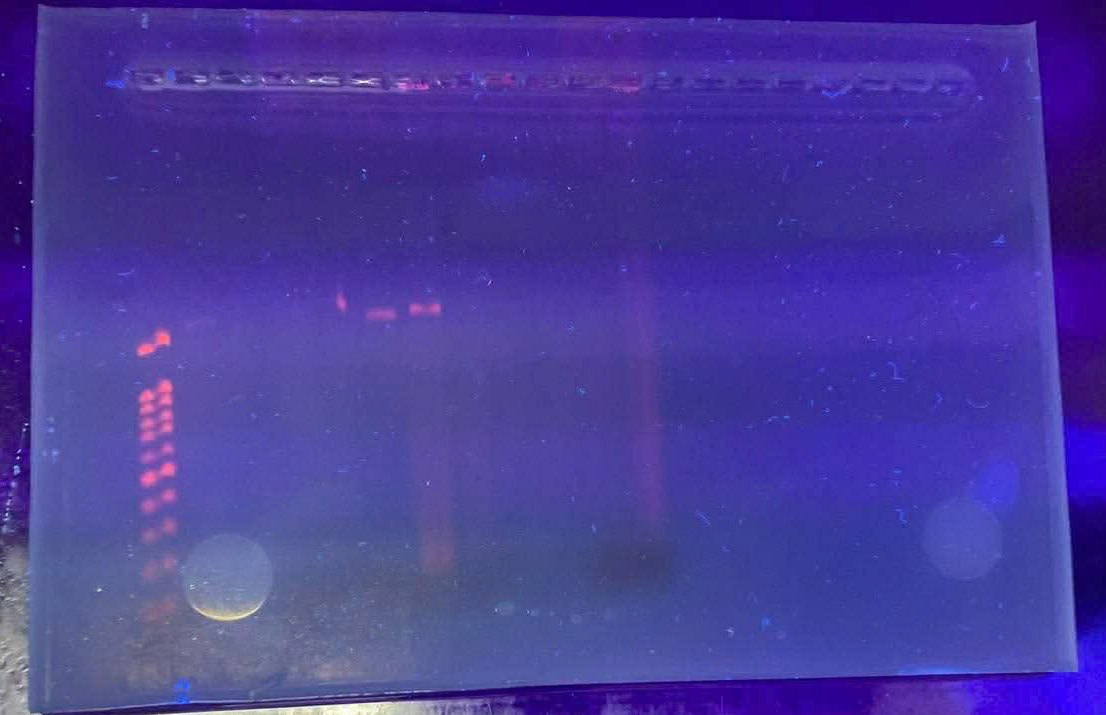
\includegraphics[width=0.8\textwidth]{Images/gel_photo.png} % Figure to be added later
\caption{Gel electrophoresis of PCR products from UV-treated bacterial DNA. Lane 1: 100 bp ladder. Lanes 4--6: bands of increasing intensity corresponding to increasing post-UV recovery time, indicating time-dependent DNA repair.}
\label{fig:gel_electrophoresis}
\end{figure}

\subsection{Lane Analysis}
\begin{itemize}
    \item \textbf{Lane 1 (100 bp DNA ladder):} The ladder resolved clearly with multiple distinct bands, confirming that gel preparation, electrophoresis, and staining were performed correctly.
    \item \textbf{Lanes 4, 5, and 6 (UV-treated samples with increasing recovery times):} Faint but visible PCR bands were observed. Notably, band intensity increased progressively from Lane 4 to Lane 6, corresponding to longer post-UV recovery times. This indicates that bacteria given more time to repair UV-induced DNA damage yielded higher-quality template DNA, resulting in more efficient PCR amplification.
    \item \textbf{Remaining sample lanes:} No discrete bands were detected. The absence of signal in these lanes is attributed to experimental errors during sample handling (see Section 5.3).
\end{itemize}

\begin{table}[h!]
\centering
\caption{Summary of Gel Electrophoresis Results}
\label{tab:results_summary}
\begin{tabular}{@{}llcc@{}}
\toprule
\textbf{Lane} & \textbf{Sample (estimated)} & \textbf{Band visible?} & \textbf{Relative intensity} \\ \midrule
1             & 100 bp ladder               & Yes --- clear          & ---                         \\
2             & Control or short recovery   & No                     & ---                         \\
3             & Control or short recovery   & No                     & ---                         \\
4             & UV-treated, moderate recovery & Yes                   & + (faint)                   \\
5             & UV-treated, longer recovery   & Yes                   & ++ (moderate)               \\
6             & UV-treated, longest recovery  & Yes                   & +++ (strongest)             \\
7+            & Other samples               & No                     & ---                         \\ \bottomrule
\end{tabular}
\end{table}

\section{Discussion}

\subsection{Expected Results}
In this experiment, bacteria were exposed to UV radiation for 30 minutes and then allowed to recover at room temperature for varying durations (15, 30, 60, 90, and 120 minutes). Two control groups received no UV treatment. After DNA extraction and PCR amplification, the following results were expected:
\begin{itemize}
    \item \textbf{Control groups (no UV):} Strong, bright PCR bands at the expected amplicon size, since undamaged genomic DNA serves as an efficient template for Taq polymerase.
    \item \textbf{UV-treated, short recovery (15--30 min):} Weak or absent PCR bands. UV-C radiation induces thymine dimers (cyclobutane pyrimidine dimers) that physically block Taq polymerase during extension, preventing successful amplification.
    \item \textbf{UV-treated, intermediate recovery (60 min):} Faint bands may begin to appear as bacterial DNA repair mechanisms (nucleotide excision repair, photoreactivation) have had time to remove some lesions.
    \item \textbf{UV-treated, long recovery (90--120 min):} Bands of moderate intensity, potentially approaching control levels, reflecting more extensive DNA repair prior to extraction.
\end{itemize}

\subsection{Interpretation of lanes 4--6: Time-Dependent DNA Repair}
The key finding of this experiment is the progressive increase in PCR band intensity across lanes 4, 5, and 6, which correspond to samples with increasing post-UV recovery time. This result is consistent with the expected biological mechanism:
\begin{itemize}
    \item UV-C radiation ($\sim$254 nm) induces cyclobutane pyrimidine dimers (CPDs) and 6-4 photoproducts in bacterial genomic DNA. These lesions distort the DNA helix and physically block Taq polymerase during PCR extension.
    \item Bacteria possess enzymatic DNA repair pathways --- most notably nucleotide excision repair (NER) --- that recognize and excise UV-induced lesions, restoring the original DNA sequence.
    \item Samples allowed longer recovery times before DNA extraction had more opportunity for repair, producing template DNA with fewer blocking lesions, and therefore amplifying more efficiently by PCR.
\end{itemize}
The gradient of band intensities (faint $\rightarrow$ moderate $\rightarrow$ strongest) directly demonstrates this time-dependent DNA repair and aligns with the expected results of the experiment.

\subsection{Absence of Bands in Other Lanes}
Several lanes showed no detectable PCR product. Possible explanations include:
\begin{itemize}
    \item \textbf{Pipetting or loading errors:} Incorrect volumes, accidental omission of template, or loss of sample during gel loading could result in empty wells.
    \item \textbf{DNA extraction variability:} The TRIzol-based DNA extraction protocol is sensitive to technique. Incomplete cell lysis, loss of pellet during ethanol washes, or over-/under-drying of the DNA pellet could lead to insufficient template for individual samples.
    \item \textbf{Sample mix-up or cross-contamination:} In a multi-group lab setting, mislabeling of tubes or accidental contamination may have affected specific samples.
    \item \textbf{Very short recovery time:} If any of the blank lanes correspond to 15-minute recovery samples, the extensive unrepaired UV damage may have been severe enough to completely prevent PCR amplification.
\end{itemize}

\section{Conclusion}
Despite technical issues with some sample lanes, the experiment successfully demonstrated the central hypothesis: bacterial DNA repair following UV exposure is time-dependent, as evidenced by the increasing PCR band intensity with longer recovery times in lanes 4--6. The intact DNA ladder confirms the electrophoresis system functioned correctly, and the trend observed is biologically meaningful and consistent with our understanding of UV mutagenesis and prokaryotic repair mechanisms.

To strengthen these findings in future experiments, the following improvements are recommended:
\begin{enumerate}
    \item Quantify extracted DNA concentration (e.g., NanoDrop) before PCR to normalize template input.
    \item Include a positive PCR control (known good template) to confirm reagent functionality.
    \item Use a dedicated genomic DNA extraction kit for more consistent yields.
    \item Run duplicate reactions per sample to distinguish true biological results from technical artifacts.
\end{enumerate}

\begin{thebibliography}{9}
\bibitem{1} Setlow, R. B. (1968). The photochemistry, photobiology, and repair of polynucleotides. \emph{Progress in Nucleic Acid Research and Molecular Biology}, 8, 257--295.
\bibitem{2} Chomczynski, P., \& Sacchi, N. (1987). Single-step method of RNA isolation by acid guanidinium thiocyanate-phenol-chloroform extraction. \emph{Analytical Biochemistry}, 162(1), 156--159.
\bibitem{3} Saiki, R. K., et al. (1988). Primer-directed enzymatic amplification of DNA with a thermostable DNA polymerase. \emph{Science}, 239(4839), 487--491.
\bibitem{4} Lee, P. Y., et al. (2012). Agarose gel electrophoresis for the separation of DNA fragments. \emph{Journal of Visualized Experiments}, (62), e3923.
\end{thebibliography}

\end{document}
